\bookchapter{Capitolo 60: Allestire l'ambiente di sviluppo — Xcode e il primo progetto}

\chapterintro{Chi vuole fare bene il lavoro, prima affili gli attrezzi. In questo capitolo montiamo la «cucina»: installare Xcode, far girare il simulatore, creare il primo progetto iOS della tua vita e poi smontare la struttura del progetto per guardarla bene. Ambiente pronto, vedrai per la prima volta il codice scritto da te trasformarsi in un pulsante su cui toccare — un istante che a molti resta in mente per tutta la vita.}

\booksection{Preparare un Mac}

Partiamo dalla soglia: lo sviluppo iOS si fa per forza su macOS. Se non hai un Mac, le strade sono tre: comprarne uno (basta anche un Mac mini o un MacBook Air di seconda mano), noleggiare per un periodo breve un Mac nel cloud, oppure leggere prima la parte 8 «Programmazione Android in pratica» (si può fare da Windows).

\begin{center}
\begin{tabularx}{\linewidth}{|X|X|X|}
\hline
\textbf{Voce di configurazione} & \textbf{Requisito minimo} & \textbf{Livello comodo (consigliato)} \tabularnewline
\hline
Chip & Apple Silicon (da M1) & M2 o più recente \tabularnewline
Memoria & 8GB & 16GB \tabularnewline
Disco & Almeno 40 GB liberi (Xcode è di corporatura robusta) & Da 256 GB in su \tabularnewline
Sistema & L'ultimo macOS & Aggiornamenti automatici sempre attivi \tabularnewline
\hline
\end{tabularx}
\end{center}

\begin{center}\small\color{gray}Configurazione di riferimento per un Mac da sviluppo (agosto 2026)\end{center}

\begin{tcbinfo}{Consiglio: puoi imparare il linguaggio anche senza Mac}
Swift Playgrounds, gratuito su iPad, insegna le basi di Swift (senza Mac); si installa perfino su iPhone. Fatti prima le dita agili sul linguaggio del capitolo 61 dentro Playgrounds e, arrivato il Mac, partirai in volo. «Affilare l'ascia non rallenta chi taglia la legna»: è proprio questo.

\end{tcbinfo}

\booksection{Installare Xcode}

Xcode è l'ambiente di sviluppo integrato ufficiale di Apple ed è gratuito. Si installa in tre passi:

\begin{enumerate}
  \item sul Mac apri App Store, cerca "Xcode" e tocca Installa — attenzione: pesa parecchi GB, scegli un'ora con la rete veloce;
  \item al primo avvio dopo l'installazione, accetta l'accordo e lascia finire i componenti (tutto in automatico);
  \item nel menu Xcode Settings Locations controlla che Command Line Tools sia selezionato — gli strumenti da riga di comando servono a molti script e strumenti di terze parti.
\end{enumerate}

\begin{tcbwarn}{Attenzione: il «gioco degli abbinamenti» tra versione e sistema}
Il nuovo Xcode spesso chiede l'ultimo macOS, mentre i Mac vecchi restano inchiodati a versioni datate. Per la pubblicazione su App Store Apple chiede di compilare con un Xcode abbastanza recente (di norma concede un periodo di respiro). Quindi non rimandare troppo gli aggiornamenti di sistema: gli sviluppatori iOS sono fra i più puntigliosi nell'inseguire le novità.

\end{tcbwarn}

\booksection{Creare il tuo primo progetto}

Apri Xcode Create New Project scegli iOS il template App, poi compila:

\begin{center}
\begin{tabularx}{\linewidth}{|X|X|X|}
\hline
\textbf{Voce di configurazione} & \textbf{Cosa inserire} & \textbf{Note} \tabularnewline
\hline
Product Name & MyFirstApp & Nome dell'app \tabularnewline
Team & Il tuo Apple ID (gratuito) & Serve per la firma, basta l'account personale \tabularnewline
Organization Identifier & com.example & Si unisce al Product Name per formare l'identificatore del pacchetto \tabularnewline
Interface & SwiftUI & Il framework principale di questo libro \tabularnewline
Language & Swift & Non serve spiegazione \tabularnewline
\hline
\end{tabularx}
\end{center}

\begin{center}\small\color{gray}Le cinque cose da compilare per creare il progetto\end{center}

Premuto Create, Xcode genera un progetto che parte subito. In alto a sinistra scegli un simulatore (per esempio iPhone 17) e tocca > per eseguire — dopo qualche secondo, sullo schermo del simulatore appare una finestra con scritto “Hello, world!”. La tua prima app iOS è appena nata.

\booksection{Anatomia del progetto: a cosa serve ogni file}

A sinistra c'è il navigatore del progetto; da principiante ti basta riconoscere questi:

\begin{center}
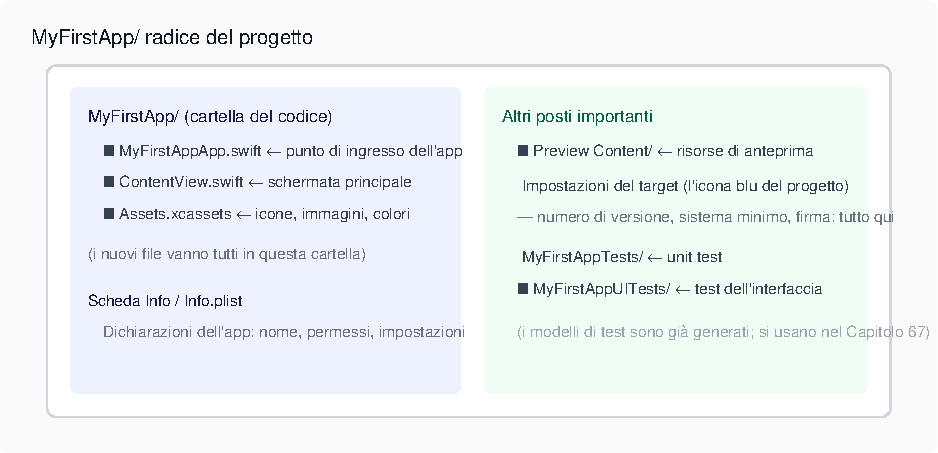
\includegraphics[width=0.92\linewidth]{figures/fig-di-liu-shi-zhang-1}
\\[2pt]\small Figura 2: la struttura del progetto Xcode che i principianti devono conoscere
\end{center}

\begin{itemize}
  \item MyFirstAppApp.swift: l'ingresso del programma, in SwiftUI sono poche righe — «avvia, poi mostra la schermata principale»;
  \item ContentView.swift: la vista della schermata principale; tutto quello che ora vedi sta qui;
  \item Assets.xcassets: il magazzino delle risorse — icone, immagini e colori stanno qui;
  \item Impostazioni del target: entra toccando l'icona blu del progetto a sinistra; dentro ci sono numero di versione, versione minima di iOS e firma. Qui si impostano anche il nome visibile dell'app e l'icona.
\end{itemize}

\booksection{Debug su dispositivo reale: portare l'app dentro il tuo iPhone}

\booksection{Trucchi di efficienza in Xcode: i cinque «potenziamenti da tastiera» per i principianti}

Imparati bene questi e sembrerai «molto professionale»:

\begin{center}
\begin{tabularx}{\linewidth}{|X|X|X|}
\hline
\textbf{Azione} & \textbf{Scorciatoia} & \textbf{A cosa serve} \tabularnewline
\hline
Eseguire & CmdR & Compila e fa girare \tabularnewline
Aprire/attivare l'anteprima nella canvas & OptionCmd & L'interruttore del WYSIWYG \tabularnewline
Sistemare l'indentazione & CtrlI & Riordina da solo l'indentazione del codice selezionato \tabularnewline
Aprire un file al volo & CmdO & Digiti il nome del file e si apre all'istante (il più usato!) \tabularnewline
Commentare/togliere il commento & Cmd/ & Attivare e disattivare righe di codice al volo durante il debug \tabularnewline
\hline
\end{tabularx}
\end{center}

\begin{center}\small\color{gray}Le scorciatoie Xcode di uso quotidiano (il corredo del principiante)\end{center}

Due benefit nascosti in più: simulatori aperti insieme (iPhone e iPad in parallelo per confrontare i layout) e la biblioteca di snippet (trascina le righe di codice di uso frequente nel pannello Snippets a destra e la volta dopo le inserisci con un tocco) — usa subito gli strumenti di efficienza e la mano si affina da sé.

\booksection{Debug su dispositivo reale: portare l'app dentro il tuo iPhone}

Il simulatore è comodo, ma il telefono vero è la meta. Con un Apple ID gratuito si può fare debug anche su dispositivo vero:

\begin{enumerate}
  \item collega l'iPhone col cavo dati (oppure fai il debug senza fili sulla stessa Wi-Fi);
  \item nell'elenco dei dispositivi in alto in Xcode scegli il tuo telefono: al primo giro chiede di accedere con l'Apple ID e prepara la firma in automatico;
  \item sull'iPhone: [Impostazioni] [Generali] [VPN e gestione dispositivi] dai fiducia al tuo certificato da sviluppatore;
  \item tocca > e l'app si installa sul telefono vero.
\end{enumerate}

\begin{tcbwarn}{Attenzione: il «limite dei sette giorni» dell'account gratuito}
Le app firmate con un Apple ID gratuito scadono dopo 7 giorni (basta eseguirle ancora una volta per rinnovarle). È il meccanismo antiabuso di Apple e per la fase di studio va più che bene; l'account sviluppatore a pagamento (99 dollari/anno) non ha questo limite — dettagli al capitolo 67.

\end{tcbwarn}

\booksection{Primo assaggio + pronto soccorso per gli errori comuni}

\booksection{Primo assaggio + pronto soccorso per gli errori comuni}

Apri ContentView.swift, sostituisci il testo dentro Text(“Hello, world!”) col tuo nome e premi CmdR per rieseguire — dopo qualche secondo sul simulatore compare il tuo nome. Congratulazioni: hai portato a termine il primo ciclo completo «modificare il codice compilare installare eseguire».

\begin{center}
\begin{tabularx}{\linewidth}{|X|X|X|}
\hline
\textbf{Errore osservato} & \textbf{Causa ricorrente} & \textbf{Rimedio} \tabularnewline
\hline
Errore di Signing & Team non scelto, certificato scaduto & In Target Signing seleziona il tuo account; con l'account gratuito esegui ancora una volta \tabularnewline
Simulatore a schermo nero / non si apre & Immagine di sistema corrotta & Menu Device Erase All Content; oppure cancella il simulatore e ricrealo \tabularnewline
Xcode scarica piano / non si installa & Rete di App Store traballante & Cambia fascia oraria; oppure scarica il pacchetto .xip offline dal sito per sviluppatori Apple \tabularnewline
\hline
\end{tabularx}
\end{center}

\begin{center}\small\color{gray}Tabella di pronto soccorso per gli errori d'ambiente dei principianti\end{center}

\begin{tcbpractice}{Mani in pasta: completa la tua checklist dei «riti dello sviluppatore»}
(1) Installa Xcode e fai girare il simulatore; (2) esegui una volta la tua app sul telefono vero e tieni lo screenshot come ricordo; (3) cambia il testo di Hello col tuo nome; (4) nelle impostazioni del target porta il nome visibile dell'app a «La mia prima app». Fatti questi quattro passi, sei una persona che ha un'opera sua.

\end{tcbpractice}

\begin{tcbsummary}{Riassunto del capitolo}
\begin{itemize}
  \item La soglia dura: Mac + Xcode; senza Mac, impara prima il linguaggio con Swift Playgrounds su iPad
  \item Xcode si installa da App Store; le versioni nuove chiedono il sistema aggiornato, non rimandare
  \item I cinque ingredienti del nuovo progetto: nome, Team, identificatore dell'organizzazione, SwiftUI, Swift
  \item La regola del progetto: tutto il codice sta nella cartella MyFirstApp/; le impostazioni del target reggono versione e firma
  \item Con l'Apple ID gratuito il debug su dispositivo vero ha il limite della firma a 7 giorni; l'account a pagamento non ce l'ha
  \item La giornata tipo dello sviluppatore = cambiare il codice CmdR guardare l'effetto, e si ricomincia
\end{itemize}

\end{tcbsummary}
